% Plantilla TFG LaTeX LSI por:
%   Agustín Borrego <borrego@us.es>
%   Inma Hernández <inmahernandez@us.es>
% Su uso y modificación es libre.

% ̀¡Recuerda hacer copias de seguridad frecuentes durante la redacción del trabajo!
% Puedes descargar todo el código fuente del proyecto en zip en Menú > (Descargar) Fuente

\documentclass[12pt]{report}

% Paquetes LaTeX y estilos globales
\input{etc/pkgs}
\input{etc/style}

%%%%%%%%%%%%%%%%%%%%%%%%%%%%%%%%%%%%%%%%%%%%%%%%%%%%%%%%%%%%%%%%%%%%%%%%%%%%%%%%%%%%%

% Variables para la portada
\setTitle{DeckBuilder una aplicacion en C con MongoDB}
\setAuthor{Borrego González, Adolfo\\ Sánchez Carmona, Germán} % Si hay más de un autor, separarlos con \\
\setDegree{Grado en Ingeniería Informática - Ingeniería del Software} % Cambiar si es necesario
\setDepartment{Lenguajes y Sistemas Informáticos}

%%%%%%%%%%%%%%%%%%%%%%%%%%%%%%%%%%%%%%%%%%%%%%%%%%%%%%%%%%%%%%%%%%%%%%%%%%%%%%%%%%%%%

% Dedicatoria del trabajo
% Si no se desea incluir, comentar o borrar la línea siguiente para eliminar la página de dedicatoria
% \setDedication{Aquí la dedicatoria del trabajo}

%%%%%%%%%%%%%%%%%%%%%%%%%%%%%%%%%%%%%%%%%%%%%%%%%%%%%%%%%%%%%%%%%%%%%%%%%%%%%%%%%%%%%

% Comienzo del documento
\begin{document}

    % Portada y secciones no numeradas
    \thispagestyle{empty} % Impide que se incluya número de página en la portada
\begin{center}

\vspace*{1cm}


\includegraphics[width=\textwidth]{figures/etsii_us.png}

\vspace*{3cm}
\begin{large}
Trabajo Complementos de Bases de Datos
\end{large}

\vspace*{0.1in}
\textbf{\huge \tfgTitle}

\vspace*{.2in}

{\large Realizado por}\\
\textbf{\Large \tfgAuthors}

\vspace*{3cm}

\textbf{Grado}\\
{\large \tfgDegree}

\vspace*{0.2in}

\textbf{Departamento de}\\
{\large \tfgDepartment}

\end{center}

% Dedicatoria
% \ifdefined\tfgDedication
%     \newpage
%     \thispagestyle{empty}
    
%     \vspace*{\fill}
%     \begin{center}
%     \textit{\tfgDedication}
%     \end{center}
%     \vspace*{\fill}
% \fi

\clearpage\setcounter{page}{1} % Comienza a incluir números de página a partir de aquí
\pagenumbering{roman} % En números romanos
    
    % Índice del documento y de figuras
    \begingroup
        % Los enlaces son normalmente azules, pero en los índices se configuran a negro para que no aparezca todo azul
        \hypersetup{linkcolor=black}
        \tableofcontents
        % \listoffigures
        % \listoftables
        % \lstlistoflistings
    \endgroup
    
    % Cambia el estilo de números de página de romanos a normal
    \clearpage\pagenumbering{arabic}
    
    % Capítulos del trabajo
    \input{sections/ejemplos_borrame.tex}
    \chapter{Introducción}\label{cap:introduccion}

En los últimos años se ha podido observar un notable crecimiento en la popularidad de los juegos de cartas coleccionables (TCG) como pueden ser Pokémon, Magic: The Gathering y Yu-Gi-Oh! Por esto surge la necesidad de usar una herramienta centralizada que permite la construcción de mazos y gestión de inventario. Este trabajo describe el diseño e implementación de DeckBuilder, una aplicación que busca facilitar e integrar las tareas de los coleccionistas.

El proyecto consiste en el desarrollo de una API REST que permita operaciones CRUD (Create, Read, Update, Delete) sobre barajas e inventarios de cartas, implementado en C\# mediante .NET 8 y usando MongoDB como base de datos. La elección de estas tecnologías, más en concreto de MongoDB, permite gestionar datos heterogéneos con estructuras y atributos variables, lo que encaja perfectamente con nuestra propuesta multijuego.

El objetivo principal del proyecto es construir una aplicación capaz registrar cartas obtenidas a través de APIs externas dedicadas \cite{tcgdexApi,scryfallApi,ygoprodeckApi}, de forma que se garantice lo máximo posible la precisión de la información. De este modo, se busca resolver la necesidad de usar múltiples aplicaciones para gestionar las colecciones de distintas franquicias.

El proyecto se estructura en tres fases:

\begin{enumerate}
    \item Planificación y Diseño
    \item Desarrollo e implementación
    \item Documentación y Presentación
\end{enumerate}

Como resultado, se ha obtenido una aplicación funcional que destaca por su capacidad de adaptarse a distintos esquemas de datos gracias al uso de bases de datos documentales.

    \chapter{Planificación y Diseño}\label{cap:planificacion}

\section{Ideas y Alcance}

Esta fase inicial fue determinante para establecer los cimientos de este proyecto. El
primer hito fue una reunión inicial de definición de alcance donde se determinó que,
para que el sistema fuera útil, debía ser capaz de manejar distintos juegos de cartas
sin reestructurar la base de datos para cada franquicia.

Durante la reunión, contemplamos diversas formas de orientar el proyecto sobre la
base de las tecnologías escogidas. Tras analizar cómo usar APIs externas para la
extracción de cartas, llegamos a la conclusión de que la creación de barajas
personalizadas era la idea con más sentido para implementar el CRUD completo que se
nos pedía. La visión era crear una base sólida que permitiera, en las siguientes
fases, mejorar la lógica interna de validación de reglas.

\section{Análisis del Flujo de Usuario y Casos de Uso}

Para que la aplicación sea operativa, se definió un flujo de usuario lineal y lógico
que maximiza la eficiencia en la gestión de colecciones. Este flujo se documentó bajo
los siguientes pasos:

\begin{itemize}
	\item \textbf{Identificación y Autenticación:} El usuario accede al sistema, lo
	que permite vincular sus barajas personalizadas a su perfil único almacenado en
	MongoDB.
	\item \textbf{Consulta y Descubrimiento:} El usuario utiliza el buscador. Este
	componente realiza peticiones a la API externa de tcgdex.dev, devolviendo el
	listado de cartas candidatas.
	\item \textbf{Persistencia en Colección:} Una vez seleccionada una carta, el
	sistema CRUD realiza una operación de creación (CREATE) para guardar la referencia
	y los metadatos específicos.
	\item \textbf{Construcción de Barajas:} El usuario crea un contenedor
	``Baraja'' donde añade y retira cartas. Aquí se aplica la lógica de edición
	(UPDATE) para modificar cantidades o estados.
	\item \textbf{Ver y Eliminar:} El usuario puede ver sus barajas, lo que sería la
	funcionalidad de (READ), y podría, si quisiera, eliminarlas con la operación de
	(DELETE).
\end{itemize}

\section{Diseño de la Arquitectura de Datos en MongoDB}

Al haber seleccionado MongoDB por el interés del equipo en las bases de datos no
relacionales, el diseño de la arquitectura fue un punto clave. A diferencia de un
modelo SQL rígido, optamos por un esquema basado en documentos BSON, lo que permite
una flexibilidad total en los atributos.

\textbf{Figura 1.} Modelo datos User (MongoDB)

\textbf{Figura 2.} Modelo datos Deck (MongoDB)

\textbf{Figura 3.} Modelo datos User\_Card (MongoDB)

\section{Stack Tecnológico}

El requisito principal del proyecto era construir una API REST que permitiese trabajar
con una base de datos NoSQL en MongoDB. Para este proyecto en concreto, teníamos la
restricción de que la tecnología a utilizar debía ser C\#, por lo que construimos el
backend en .NET 8. Este se encarga de la lógica de negocio y exponer la API.

Por otro lado, para ampliar el alcance inicial, se decidió incluir una capa frontend
mediante React + Vite + TypeScript, con el objetivo de facilitar el uso de la API de
cara a los usuarios.

En cuanto a infraestructura, el proyecto se desplegó en servicios cloud:

\begin{itemize}
	\item Render para backend y frontend.
	\item MongoDB Atlas para alojar la base de datos en entorno gestionado.
\end{itemize}

De esta forma, la solución mantiene el núcleo requerido (MongoDB + C\#) y añade una
arquitectura web completa, preparada para uso real y validación en producción.

\section{Resultado de la fase}

La fase de planificación y diseño ha permitido establecer una base sólida para el
desarrollo del proyecto. Durante esta etapa se han definido claramente los objetivos
del sistema, el alcance funcional y el flujo de usuario, asegurando que la aplicación
cubra las necesidades principales de gestión de barajas.

Como resultado de esta fase, se ha obtenido una visión clara del funcionamiento global
del sistema, incluyendo la interacción entre usuario, aplicación y fuentes externas de
datos. Además, ha quedado definido el stack tecnológico. Esto ha facilitado la
transición hacia la fase de desarrollo, donde se ha podido implementar el sistema de
manera más eficiente y con menor riesgo de errores estructurales.

    \chapter{Desarrollo e Implementación}\label{cap:desarrollo}

\section{Implementación del núcleo funcional}

Esta segunda etapa del proyecto se centró en la transformación de los diseños y
esquemas previos en un producto de software funcional. El objetivo primordial
consistió en construir una base tecnológica sólida que cubriera el ciclo de vida
completo del usuario dentro de la aplicación: desde el proceso de autenticación
inicial hasta la gestión avanzada de sus barajas.

Para asegurar la calidad del software, la implementación se llevó a cabo de forma
incremental y modular. Este enfoque, basado en el cumplimiento de hitos concretos y el
uso de commits atómicos, permitió validar de manera constante cada funcionalidad antes
de proceder a la siguiente, minimizando el riesgo de errores estructurales.

\section{Implementación del backend}

En el entorno de backend, se estructuró una API bajo el entorno de .NET 8 diseñada
para soportar operaciones sobre las barajas de usuarios autenticados.
Durante este proceso, se priorizó la separación de responsabilidades mediante el uso
de DTOs y validaciones independientes, lo que mejora la mantenibilidad del código y
evita el acoplamiento entre la lógica de negocio y la capa de transporte de datos.

Sobre esta arquitectura se consolidó el sistema CRUD completo para la entidad de
barajas: creación (CREATE), lectura (READ), actualización (UPDATE) y borrado (DELETE).
La lógica de actualización fue algo más compleja, ya que incluye la persistencia
dinámica de cartas dentro de cada mazo y la implementación de reglas de dominio
específicas, como el control de copias máximas permitidas y el tamaño total de la
baraja (60 cartas en total, con límites por nombre según juego).

Para garantizar la estabilidad de los datos externos se optimizó la comunicación con
los proveedores de cartas mediante el desarrollo de un mejor cliente HTTP. Se
realizaron ajustes pequeños en los algoritmos de búsqueda para asegurar que las
respuestas obtenidas desde fuentes como Pokémon o Magic fueran consistentes y
estuvieran listas para su procesamiento en el servidor.

Los extractos de código \ref{cod:dev-models-short},
\ref{cod:dev-controller-short} y \ref{cod:dev-validator-short} muestran,
respectivamente, un ejemplo de modelo, un endpoint de controlador y una validación de
reglas de baraja.

En el primer fragmento se observa cómo se modela una baraja en MongoDB con sus campos
clave: nombre, tipo de juego, lista de cartas y marca temporal de actualización.

\begin{lstlisting}[language={[Sharp]C}, caption={Fragmento de modelo Deck (C\#)}, label={cod:dev-models-short}, captionpos=b]
public sealed class Deck
{
    public string Name { get; set; } = string.Empty;
    public string GameType { get; set; } = DeckGameTypes.Pokemon;
    public List<DeckCard> Cards { get; set; } = new();
    public DateTime UpdatedAtUtc { get; set; } = DateTime.UtcNow;
}
\end{lstlisting}

El segundo fragmento resume el flujo básico del endpoint de creación: validar la
entrada, persistir en la colección y devolver la respuesta HTTP con el recurso creado.

\begin{lstlisting}[language={[Sharp]C}, caption={Fragmento de controlador para crear baraja (C\#)}, label={cod:dev-controller-short}, captionpos=b]
[HttpPost]
public async Task<IActionResult> CreateDeck([FromBody] CreateDeckRequest request)
{
    if (!DeckRequestValidator.TryValidateCreate(request, out var error))
        return BadRequest(new { message = error });

    await GetDecksCollection().InsertOneAsync(deck);
    return Created($"/api/decks/{deck.Id}", deck);
}
\end{lstlisting}

El tercer fragmento recoge dos de las reglas más relevantes del dominio: límite total
de cartas por baraja y número máximo de copias por nombre.

\begin{lstlisting}[language={[Sharp]C}, caption={Fragmento de validación de reglas de baraja (C\#)}, label={cod:dev-validator-short}, captionpos=b]
if (totalCards > MaxCardsPerDeck)
{
    errorMessage = $"Una baraja no puede superar {MaxCardsPerDeck} cartas.";
    return false;
}

if (copiesByName[normalizedName] > maxCopiesPerName)
{
    errorMessage = $"No puedes tener mas de {maxCopiesPerName} copias con el mismo nombre.";
    return false;
}
\end{lstlisting}

La API desarrollada sigue un diseño REST, estructurado en torno a recursos como
usuarios, barajas y cartas. Esta organización permite una separación clara de
responsabilidades y facilita la escalabilidad del sistema.

\subsection*{Documentación de la API}

Los endpoints implementados cubren tanto la autenticación como la gestión completa de
barajas, la colección de cartas del usuario y la comprobación del servicio.

\subsubsection*{Comprobación del servicio}

\begin{itemize}
	\item GET /: estado básico del backend.
	\item GET /api/health/mongo: comprobación de conectividad con MongoDB.
\end{itemize}

\subsubsection*{Autenticación}

\begin{itemize}
	\item POST /api/auth/register: registro nuevos usuarios.
	\item POST /api/auth/login: autenticación de usuarios existentes.
	\item DELETE /api/auth/me: eliminación de la cuenta autenticada y sus datos
	asociados.
\end{itemize}

\subsubsection*{Gestión de barajas (Decks)}

\begin{itemize}
	\item GET /api/decks: obtención de todas las barajas del usuario autenticado.
	\item GET /api/decks/\{deckId\}: consulta detallada de baraja específica.
	\item POST /api/decks: creación de nueva baraja.
	\item PUT /api/decks/\{deckId\}: actualización de una baraja, incluyendo
	modificar cartas.
	\item DELETE /api/decks/\{deckId\}: eliminación de una baraja.
\end{itemize}

\subsubsection*{Búsqueda de cartas}

\begin{itemize}
	\item GET /api/cards/search: búsqueda de cartas en fuentes externas.
\end{itemize}

\subsubsection*{Gestión de colección de cartas (User Cards)}

\begin{itemize}
	\item GET /api/user-cards: obtención de la colección de cartas del usuario,
	con filtros opcionales.
	\item GET /api/user-cards/stats: obtención de estadísticas de colección,
	con posibilidad de filtrar por juego.
	\item POST /api/user-cards: inserción de nuevas cartas en colección.
	\item POST /api/user-cards/\{userCardId\}/quantity: ajuste incremental de copias
	carta.
	\item DELETE /api/user-cards/\{userCardId\}: eliminación de carta de colección.
\end{itemize}

Este conjunto de endpoints constituye la base del sistema CRUD ampliado, no solo
sobre barajas sino también sobre la colección personal del usuario. La inclusión de
endpoints de estadística y búsqueda externa aporta un valor añadido al sistema.

Su funcionamiento detallado y configuración se encuentran descritos en el archivo
README del repositorio, donde se abordan aspectos como la lógica de interacción,
validaciones y comunicación con la base de datos.

\section{Implementación del frontend y flujo operativo}

Paralelamente, el desarrollo de la interfaz de usuario evolucionó desde prototipos
estáticos hacia un flujo operativo completo y dinámico. Se implementó un sistema de
gestión de sesiones que permite el cambio fluido entre las vistas de registro e inicio
de sesión, garantizando que el usuario acceda únicamente a su colección privada
almacenada en MongoDB una vez identificado.

Tras la validación del acceso, se desarrollaron las vistas de colección y el detalle
de cada baraja. Estas interfaces permiten al usuario interactuar en tiempo real con su
contenido, editando la composición del mazo y persistiendo los cambios de forma
inmediata con la API. Esta evolución incluye una refactorización integral del cliente
por áreas de responsabilidad (autenticación, colección y comunicación con la API) para
facilitar la escalabilidad futura.

Como fase de cierre de la interfaz, se incorporó la funcionalidad de borrado
definitivo de barajas y se aplicaron técnicas de diseño responsive. Estas mejoras
aseguran que la experiencia de usuario sea óptima y visualmente coherente en una
amplia variedad de dispositivos.

Las principales pantallas del frontend pueden verse en la Figura
\ref{fig:dev-frontend-lista-barajas}, la Figura
\ref{fig:dev-frontend-mi-coleccion}, la Figura
\ref{fig:dev-frontend-detalles-baraja} y la Figura
\ref{fig:dev-frontend-buscador}.

\begin{figure}[H]
	\centering
	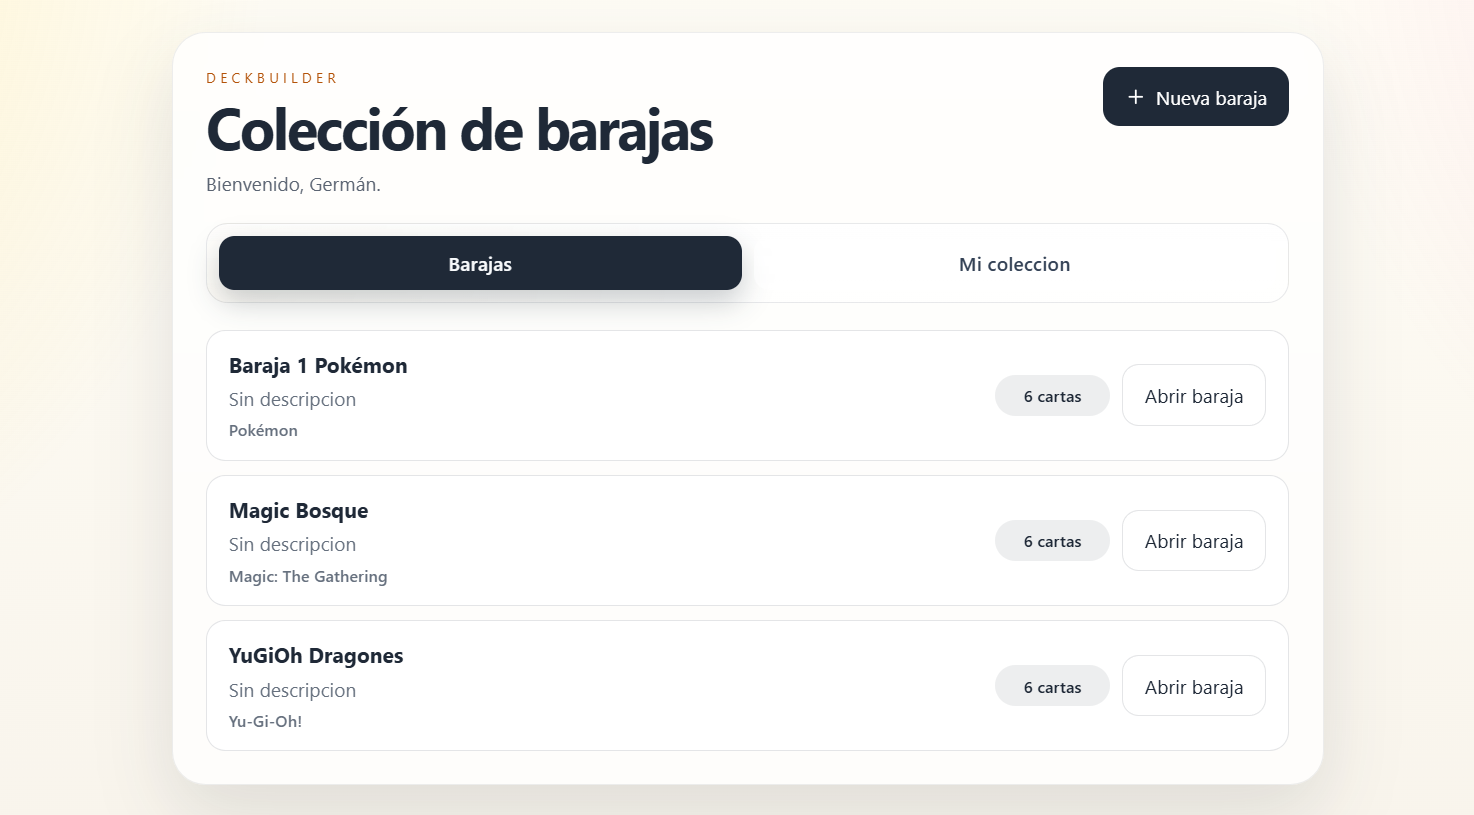
\includegraphics[width=0.9\textwidth]{figures/lista-barajas.png}
	\caption{Pantalla de colección de barajas}
	\label{fig:dev-frontend-lista-barajas}
\end{figure}

\begin{figure}[H]
	\centering
	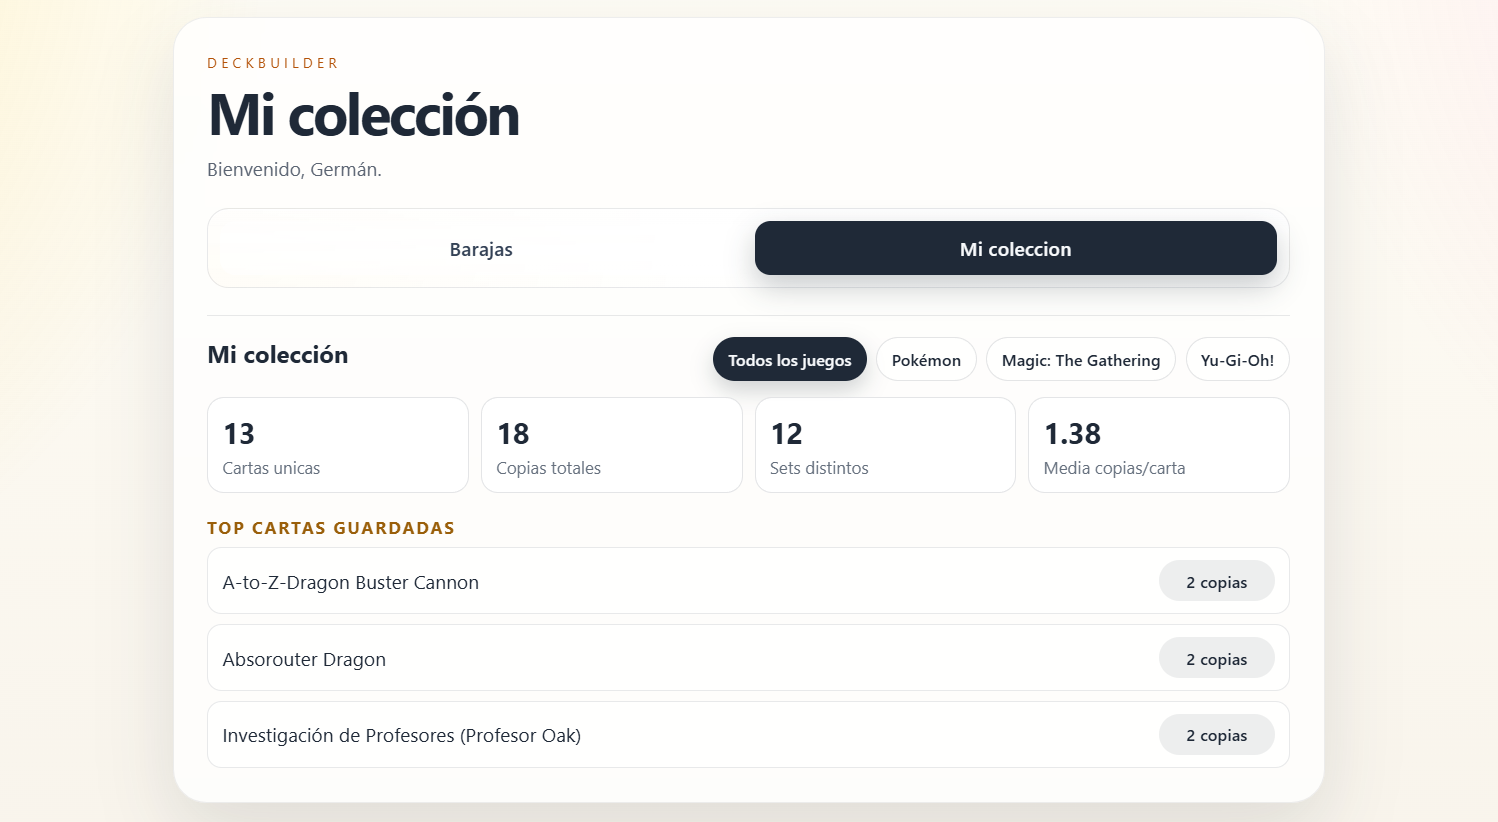
\includegraphics[width=0.9\textwidth]{figures/mi-coleccion.png}
	\caption{Pantalla de Mi colección}
	\label{fig:dev-frontend-mi-coleccion}
\end{figure}

\begin{figure}[H]
	\centering
	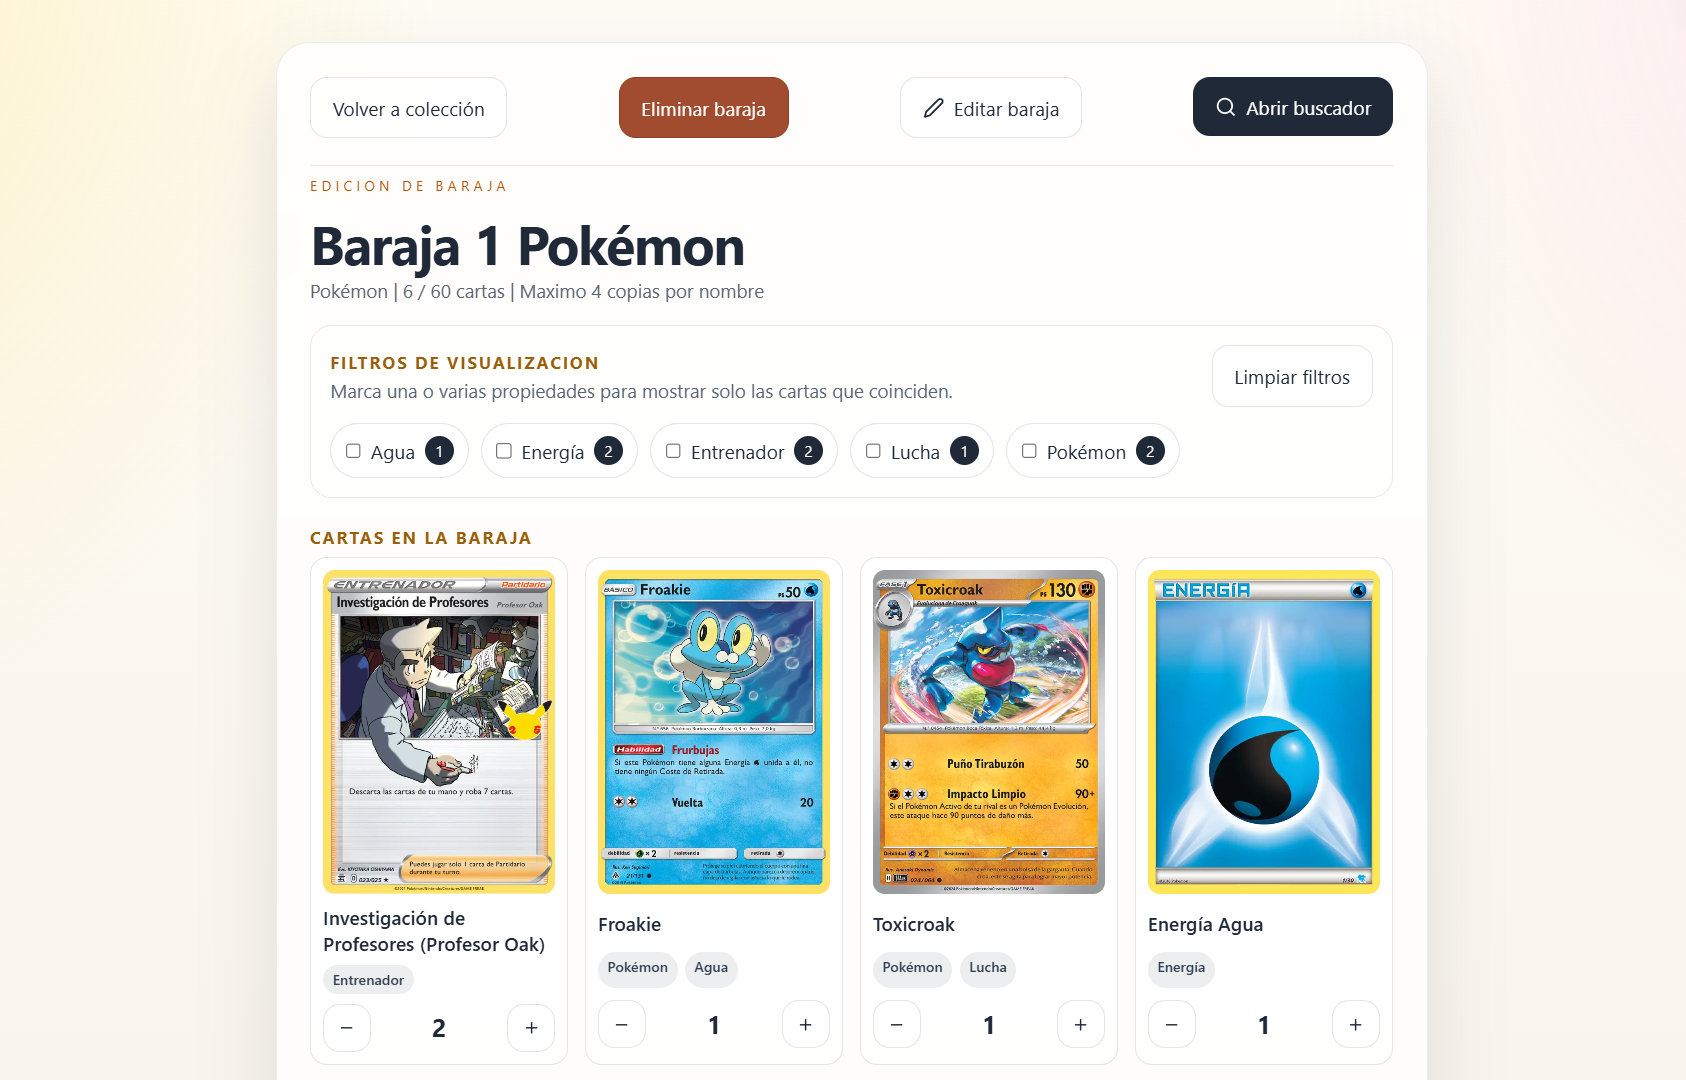
\includegraphics[width=0.9\textwidth]{figures/detalles-baraja.png}
	\caption{Pantalla de detalle y edición de baraja}
	\label{fig:dev-frontend-detalles-baraja}
\end{figure}

\begin{figure}[H]
	\centering
	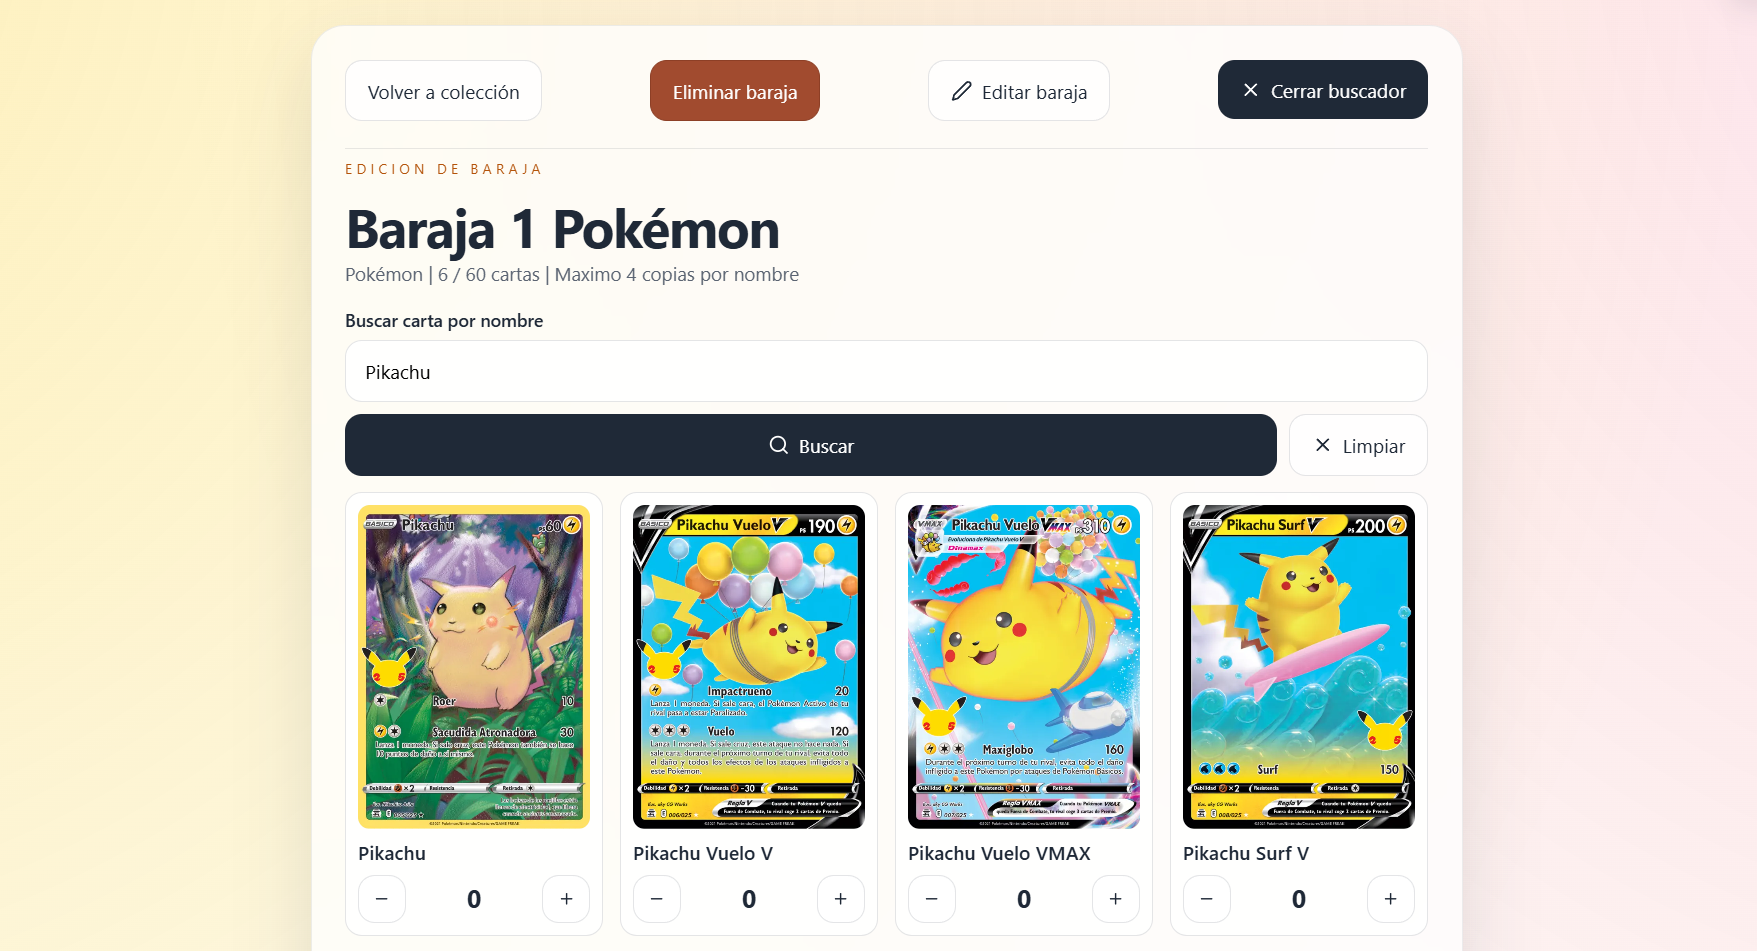
\includegraphics[width=0.9\textwidth]{figures/buscador.png}
	\caption{Pantalla de buscador de cartas}
	\label{fig:dev-frontend-buscador}
\end{figure}

\section{Capacidades multijuego y editor visual}

Una de las partes más relevantes de esta fase fue la transformación de la plataforma
en una solución multijuego auténtica. Se integra el tipo de juego (Pokémon, Magic o
Yu-Gi-Oh!) como un atributo estructural dentro de la base de datos de MongoDB,
permitiendo que el sistema se adapte dinámicamente según la elección del usuario al
crear una nueva baraja.

Gracias a esta base polimórfica, se desarrolló un endpoint de búsqueda unificado capaz
de consultar múltiples fuentes externas de manera homogénea. Esta integración permite
al usuario buscar cartas de diferentes franquicias bajo un mismo estándar visual,
simplificando la complejidad técnica de las diferentes estructuras de datos de origen.

Finalmente, se construyó el editor visual de barajas, la herramienta central de la
aplicación. En este componente, los usuarios pueden añadir o retirar cartas mediante
controles directos, mientras el sistema aplica automáticamente las reglas de validación
específicas de cada juego dentro de la lógica de actualización, garantizando que el
mazo resultante sea legal dentro de cada uno de los juegos.

El extracto \ref{cod:dev-multijuego-busqueda} resume la base de la implementación
multijuego: definir tipos de juego normalizados y seleccionar el proveedor de búsqueda
en función del valor recibido.

\begin{lstlisting}[language={[Sharp]C}, caption={DeckGameTypes simplificado y selección de proveedor (C\#)}, label={cod:dev-multijuego-busqueda}, captionpos=b]
public static class DeckGameTypes
{
    public const string Pokemon = "pokemon";
    public const string Magic = "magic";
    public const string Yugioh = "yugioh";
}

var cards = normalizedGameType switch
{
    DeckGameTypes.Pokemon => await SearchPokemonCardsAsync(httpClient, query, cancellationToken),
    DeckGameTypes.Magic => await SearchMagicCardsAsync(httpClient, query, cancellationToken),
    DeckGameTypes.Yugioh => await SearchYugiohCardsAsync(httpClient, query, cancellationToken),
    _ => []
};
\end{lstlisting}

\section{Resultados de la fase}

La Fase 2 concluyó exitosamente con un núcleo funcional operativo que integra
autenticación, vinculación de datos por usuario, un CRUD completo y un motor
multijuego. El sistema ha demostrado su funcionamiento al permitir la construcción de
mazos completos de forma muy clara e interactiva.

Desde el punto de vista arquitectónico, la solución queda preparada para crecer sin
necesidad de reestructurar la base de datos para cada nueva franquicia. Se ha logrado
una separación clara entre la interfaz, la lógica de negocio y la capa de persistencia,
dejando una base sólida para las próximas etapas.

    \chapter{Documentación y Presentación}\label{cap:documentacion}

\section{Elaboración de la documentación técnica}

La tercera fase del proyecto se ha dedicado íntegramente a la consolidación de toda
la información generada durante el ciclo de vida del desarrollo para cumplir con los
requisitos de evaluación de la asignatura. El núcleo de esta fase es la redacción de
la presente memoria, un documento que no solo describe el producto final, sino que
justifica cada decisión tomada por el equipo, desde la elección del stack
tecnológico hasta la implementación de las reglas de negocio con las barajas.

Esta labor de documentación ha permitido realizar una reflexión crítica sobre el
trabajo realizado, asegurando que todo lo alcanzado en las fases anteriores quede
registrado. La memoria actúa como el soporte principal que demuestra la adquisición de
competencias en el uso de C\# y MongoDB, detallando cómo se ha resuelto el problema de
la variabilidad de datos mediante un sistema CRUD eficiente y escalable.

\section{Preparación de la presentación}

Un componente fundamental de esta etapa ha sido la preparación de la presentación
requerida para la asignatura. Este proceso ha consistido en sintetizar los aspectos
más relevantes del desarrollo de DeckBuilder para su exposición. Se han diseñado
materiales visuales que destacan los puntos fuertes de la aplicación, como la
integración de las APIs externas y la flexibilidad de la base de datos documental.

El objetivo de esta tarea es comunicar de forma clara y concisa los resultados
obtenidos y demostrar que el núcleo funcional desarrollado en la fase anterior es
operativo y responde a los objetivos planteados al inicio.

\section{Desarrollo del archivo README: Manual usuario y despliegue}

Como cierre técnico del proyecto, se ha elaborado un archivo README dentro del
repositorio del código fuente. Este documento se ha diseñado para cumplir una doble
función: servir como manual de usuario y como guía detallada de despliegue e
instalación. En él se explican paso a paso las instrucciones necesarias para que
cualquier usuario pueda configurar el entorno de ejecución, incluyendo la vinculación
con MongoDB, la instalación de dependencias de .NET 8 y el arranque del frontend.

Además de las instrucciones técnicas, el README incluye una guía de uso que describe
el flujo operativo de la aplicación y los enlaces de acceso al despliegue en Render.

\section{Resultados finales de la fase}

La conclusión de esta fase marca el fin del desarrollo de DeckBuilder. Con la memoria
técnica finalizada, la presentación preparada y el archivo README configurado, el
proyecto queda listo para su entrega definitiva. El resultado es una aplicación que
funciona de forma correcta, respaldada por una documentación para entender todo lo
realizado.

    \chapter{Conclusiones}\label{cap:conclusiones}

Tras finalizar el desarrollo de Deckbuilder hemos logrado cumplir el objetivo principal que era diseñar e implementar una aplicación funcional que utiliza las tecnologías de C\# y MongoDB.

Una de las características más importantes del proyecto ha sido el uso de una base de datos documental. Gracias al uso de MongoDB hemos podido gestionar de la mejor forma la variabilidad de los datos entre los distintos juegos de cartas que hemos usado, evitando de esta forma las limitaciones de los modelos relaciones que conocemos.

Viéndolo desde un punto de vista técnico, el desarrollo de un CRUD completo, junto con el frontend interactivo, nos ha permitido cubrir todo el flujo del usuario dentro de la aplicación, desde la autenticación hasta la gestión completa de las barajas y colecciones.

En conclusión, el proyecto nos ha permitido aplicar de forma práctica los conceptos estudiados en la asignatura, especialmente en el uso de bases de datos NoSQL, consolidando de esta forma una buena base con estas nuevas tecnologías.


    % Bibliografía
    \bibliographystyle{unsrtnat}
    \bibliography{bibliografia.bib}

% Fin del documento
\end{document}
